% import packages
\documentclass[8pt,table=xcolor,usenames,dvipsnames]{beamer}
\usepackage[utf8]{inputenc}
\usepackage{colortbl}
\usepackage{ragged2e}
\usepackage{booktabs}
\usepackage{threeparttable}
\usepackage{pifont}
\usepackage{graphicx}
\usepackage{hhline}
\usepackage{amsmath}
\usepackage{amssymb}
\usepackage{amsthm}
\usepackage{tikz}
\usepackage{bm}
\usepackage[export]{adjustbox}
\usepackage[justification=centering]{caption}
\usepackage[backend=bibtex,style=authoryear,maxcitenames=2,natbib=true,maxbibnames=99]{biblatex}

% set beamer parameters
\usetheme{Frankfurt}
\usecolortheme{default}
\setbeamerfont{footnote}{size=\Tiny}
\setbeamertemplate{page number in head/foot}{}
\setbeamertemplate{bibliography item}{}
\setbeamertemplate{caption}[numbered]
\setbeamercovered{transparent}
\setbeamerfont{institute}{size=\small}
\addtobeamertemplate{navigation symbols}{}{%
  \usebeamerfont{footline}%
  \usebeamercolor[fg]{footline}%
  \hspace{2em}%
  \raisebox{1.7pt}[0pt][0pt]{\insertframenumber/\inserttotalframenumber}
}
\setbeamertemplate{enumerate items}[square]
\setbeamertemplate{section in toc}[square]
\setbeamertemplate{theorems}[numbered]

% special command to uncover graphics
% source: https://tex.stackexchange.com/a/415335
\newcommand<>{\uncovergraphics}[2][{}]{
  % Taken from: <https://tex.stackexchange.com/a/354033/95423>
  \begin{tikzpicture}
    \node[anchor=south west,inner sep=0] (B) at (4,0)
    {\includegraphics[#1]{#2}}; \alt#3{}{%
      \fill [draw=none, fill=white, fill opacity=0.7] (B.north west) -- (B.north
      east) -- (B.south east) -- (B.south west) -- (B.north west) -- cycle; }
  \end{tikzpicture}
}

% set caption parameters
\DeclareCaptionFormat{myformat}{\fontsize{6}{6}\selectfont#1#2#3}
\captionsetup{format=myformat}
\captionsetup[figure]{labelfont={bf},name={Figure}}
\captionsetup[table]{labelfont={bf},name={Table}}

% set bibliography parameters
\renewcommand\refname{Bibliography}
\addbibresource{../bibtex.bib}
\setlength\bibitemsep{1.5\itemsep}
\let\oldcitep=\citep
\renewcommand\citep[1]{{\textcolor{blue}{\oldcitep{#1}}}}
\let\oldcitet=\citet
\renewcommand\citet[1]{{\textcolor{blue}{\oldcitet{#1}}}}

% miscellaneous settings
\settowidth{\leftmargini}{\usebeamertemplate{itemize item}}
\addtolength{\leftmargini}{\labelsep}
\renewcommand{\arraystretch}{1.3}
\graphicspath{{../visuals/}}
\newcolumntype{L}[1]{>{\RaggedRight\hspace{0pt}}p{#1}}

% set admin details
\title{SoPa++: Leveraging explainability from hybridized RNN, CNN and weighted
  finite-state neural architectures}
\subtitle{M.Sc. Thesis Defense}
\author{Atreya Shankar (799227), \texttt{shankar.atreya@gmail.com} \\ Cognitive Systems:
  Language, Learning, and Reasoning (M.Sc.) \\ 1\textsuperscript{st} Supervisor: Dr. Sharid
  Loáiciga, University of Potsdam \\ 2\textsuperscript{nd}
  Supervisor: Mathias Müller, M.A., University of Zurich}
\institute{Foundations of Computational Linguistics \\ Department of Linguistics \\ University of Potsdam, SoSe 2021}
\date{July 8, 2021}

% start presentation
\begin{document}
\begin{frame}
  \maketitle
\end{frame}

\begin{frame}
  \frametitle{Overview}
  \tableofcontents
\end{frame}

\section{Introduction}

\begin{frame}
  \frametitle{Motivation}

  \begin{columns}[T]
    \begin{column}{.40\textwidth}
      \begin{itemize}
        \setlength\itemsep{1em}
        \uncover<1>{
          \item Trend of increasingly complex deep learning models achieving
          SOTA performance on ML and NLP tasks (Figure \ref{fig:nlp_progress})
          \item To address emerging concerns such as inductive biases, several
          studies make arguments for research into XAI; for example
          \citet{danilevsky2020survey} and \citet{arrieta2020explainable}}
        \uncover<2>{
          \item \citet{schwartz2018sopa} approach XAI in NLP by proposing an
          explainable hybridized neural architecture called \textbf{So}ft
          \textbf{Pa}tterns (SoPa; Figure \ref{fig:sopa_crop})
          \item SoPa provides \textbf{localized} and \textbf{indirect} explainability despite
          being suited for globalized and direct \textbf{explanations by
            simplification}
        }
      \end{itemize}
    \end{column}
    \hfill
    \begin{column}{.60\textwidth}
      \centering
      \uncovergraphics<1>[width=6cm, valign=t]{pdfs/borrowed/nlp_sota_model_size_progress.pdf}
      \uncover<1>{\captionof{figure}{Parameter counts of recently released pre-trained language
          models; figure taken from \citet{sanh2019distilbert}}}
      \label{fig:nlp_progress}
      \vspace{10pt}
      \uncover<2>{\fbox{\uncovergraphics<2>[width=6cm, valign=t]{pdfs/borrowed/sopa_crop.pdf}}}
      \uncover<2>{\captionof{figure}{Excerpt from \citet{schwartz2018sopa}}}
      \label{fig:sopa_crop}
    \end{column}
  \end{columns}
\end{frame}

\begin{frame}
  \frametitle{Objective and research questions}

  \uncover<1->{ Objective: \setlength{\leftmargini}{0.5cm}
    \begin{itemize}
      \item Address limitations of SoPa by proposing \textbf{SoPa++}, which
      could allow for effective explanations by simplification
    \end{itemize}
  }
  
  \vspace{10pt}

  \uncover<2->{ Process:
    \begin{itemize}
      \item We study the performance and explanations by simplification of
      SoPa++ on the Facebook Multilingual Task Oriented Dialog (\textbf{FMTOD}) data set from
      \citet{schuster-etal-2019-cross-lingual}; focusing on the English-language
      intent classification task.
    \end{itemize}
  }
  
  \vspace{10pt}

  \uncover<3->{ Research questions:
    \begin{enumerate}
      \setlength\itemsep{1em}
      \item Does SoPa++ provide \textbf{competitive} performance?
      \item To what extent does SoPa++ contribute to \textbf{effective}
      explanations by simplification?
      \item What \textbf{interesting and relevant} explanations can SoPa++
      provide?
    \end{enumerate}
  }
\end{frame}

% macro for showing TOC on each new section
\AtBeginSection[]
{
  \begin{frame}
    \frametitle{Overview}
    \tableofcontents[currentsection]
  \end{frame}
}

\section{Background concepts}

\begin{frame}
  \frametitle{Explainability}
  \begin{columns}[T]
    \begin{column}{.40\textwidth}
      \begin{itemize}
        \setlength\itemsep{1em}
        \uncover<1>{
          \item Transparency is a passive feature that a model exhibits
          \item Explainability is an active feature that involves target
          audiences (Figure \ref{fig:xai_target_audience})
          \item \citet{arrieta2020explainable} explore a taxonomy of post-hoc
          explainability techniques}
        \uncover<2>{
          \item Explainability techniques can provide meaningful insights into
          decision boundaries within black-box models (Figure
          \ref{fig:lime_husky})
          \item Prominent explainability techniques include local
          explanations, feature relevance and \textbf{explanations by
            simplification}
        } 
      \end{itemize}
    \end{column}
    \hfill
    \begin{column}{.60\textwidth}
      \centering
      \uncovergraphics<1>[width=6.2cm,trim={0.3cm 0.3cm 0.5cm
        0.3cm},clip,valign=t]{pdfs/borrowed/xai_target_audience.pdf}
      \uncover<1>{\captionof{figure}{Examples of various target audiences in XAI; figure taken from
          \citet{arrieta2020explainable}}}
      \label{fig:xai_target_audience}
      \vspace{5pt}
      \uncovergraphics<2>[width=6cm,trim={0.1cm 0.1cm 0.1cm
        0.1cm},clip,valign=t]{pdfs/borrowed/lime_husky.pdf}
      \uncover<2>{\captionof{figure}{Local explanation for ``Wolf''
          classification decision, figure taken from \citet{lime}}}
      \label{fig:lime_husky}
    \end{column}
  \end{columns}
\end{frame}

\begin{frame}
  \frametitle{SoPa: Weighted Finite-State Automaton (WFA)}
  \uncover<1>{\begin{definition}[Semiring; \citealt{kuich1986linear}]
      \label{def:semiring}
      A semiring is a set $\mathbb{K}$ along with two binary associative
      operations $\oplus$ (addition) and $\otimes$ (multiplication) and two
      identity elements: $\bar{0}$ for addition and $\bar{1}$ for
      multiplication. Semirings require that addition is commutative,
      multiplication distributes over addition, and that multiplication by
      $\bar{0}$ annihilates, i.e., $\bar{0} \otimes a = a \otimes \bar{0} =
      \bar{0}$.

      \begin{itemize}
        \item Semirings follow the following generic notation: $\langle
        \mathbb{K}, \oplus, \otimes, \bar{0}, \bar{1} \rangle$.
        \item \textbf{Max-sum} semiring: $\langle \mathbb{R} \cup \{-\infty\},
        \text{max}, +, -\infty, 0 \rangle$
        \item \textbf{Max-product} semiring: $\langle \mathbb{R}_{>0} \cup
        \{-\infty\}, \text{max}, \times, -\infty, 1 \rangle$
      \end{itemize}
    \end{definition}}

  \uncover<2>{\begin{definition}[Weighted finite-state automaton;
      \citealt{peng2018rational}]
      \label{def:wfa}
      A weighted finite-state automaton over a semiring $\mathbb{K}$ is a
      5-tuple $\mathcal{A} = \langle \Sigma, \mathcal{Q}, \bm{\Gamma},
      \bm{\lambda}, \bm{\rho} \rangle$, with:

      \begin{itemize}
        \itemsep0em
        \item[--] a finite input alphabet $\Sigma$;
        \item[--] a finite state set $\mathcal{Q}$;
        \item[--] transition matrix $\bm{\Gamma}: \mathcal{Q} \times \mathcal{Q}
        \times (\Sigma \cup \{\epsilon\}) \rightarrow \mathbb{K}$;
        \item[--] initial vector $\bm{\lambda}: \mathcal{Q} \rightarrow
        \mathbb{K}$;
        \item[--] and final vector $\bm{\rho}: \mathcal{Q} \rightarrow
        \mathbb{K}$.
      \end{itemize}
    \end{definition}}
\end{frame}

\begin{frame}
  \frametitle{SoPa: Computational graph}
  \centering
  \captionsetup{width=9cm}
  \uncovergraphics<1->[width=8cm, valign=t]{pdfs/generated/generic_nfa_linear_chain/main.pdf}
  \uncover<1->{\captionof{figure}{WFA slice: linear-chain FA with
      self-loop (blue), $\epsilon$ (red) and main-path (black) transitions; figure
      adapted from \citet{schwartz2018sopa}}}
  \label{fig:fa}
  \vspace{10pt}
  \uncovergraphics<2>[width=8cm, valign=t]{pdfs/borrowed/sopa_computational_graph.pdf}
  \uncover<2>{\captionof{figure}{SoPa's partial computational graph; figure taken from
      \citet{schwartz2018sopa}}}
  \label{fig:sopa}
\end{frame}

\begin{frame}
  \frametitle{SoPa: Post-hoc explainability techniques}
  \begin{columns}[T]
    \begin{column}{.40\textwidth}
      \begin{itemize}
        \setlength\itemsep{1.4em}
        \uncover<1->{
          \item SoPa provides two post-hoc explainability techniques; namely
          \textbf{local explanations} and \textbf{feature relevance}
          \item Local explanations gather highest scoring phrases across the
          training data (Figure \ref{fig:sopa_local_explanations})
        }
        \uncover<2>{
          \item Feature relevance perturbs inputs using an occlusion technique
          to determine the highest impact phrases for a classification decision
          (Figure \ref{fig:sopa_feature_relevance})
          \item Overall, both techniques are \textbf{localized} and
          \textbf{indirect}
          \item WFAs have a rich theoretical background which can be exploited
          for more direct and globalized explanations
        }
      \end{itemize}
    \end{column}
    \hfill
    \begin{column}{.60\textwidth}
      \centering
      \uncovergraphics<1->[width=6cm,valign=t]{pdfs/borrowed/sopa_local_explanations.pdf}
      \uncover<1->{\captionof{figure}{Ranked local explanations from SoPa;
          table taken from \citet{schwartz2018sopa}}}
      \label{fig:sopa_local_explanations}
      \vspace{5pt}
      \uncovergraphics<2>[width=6cm,trim={0cm 2.3cm 0cm
        0cm},clip,valign=t]{pdfs/borrowed/sopa_feature_relevance.pdf}
      \uncover<2>{\captionof{figure}{Feature relevance outputs from SoPa;
          table taken from \citet{schwartz2018sopa}}}
      \label{fig:sopa_feature_relevance}
    \end{column}
  \end{columns}
\end{frame}

\section{Data and methodologies}

\begin{frame}
  \frametitle{FMTOD: Summary statistics}
  \begin{table}
    \small
    \centering
    \begin{threeparttable}
      \begin{tabular}{llll}
        \toprule
        Class and description & \uncover<3>{Frequency} & \uncover<2->{Utterance length$^{\dagger}$ & Example$^{\ddagger}$}\\
        \midrule
        0: \texttt{alarm/cancel\_alarm} & \uncover<3>{\cellcolor{red!5}1791} & \uncover<2->{5.6 $\pm$ 1.9 & cancel weekly alarm} \\
        1: \texttt{alarm/modify\_alarm} & \uncover<3>{\cellcolor{red!2}566} & \uncover<2->{7.1 $\pm$ 2.5 & change alarm time} \\
        2: \texttt{alarm/set\_alarm} & \uncover<3>{\cellcolor{red!17}5416} & \uncover<2->{7.5 $\pm$ 2.5 & please set the new alarm} \\
        3: \texttt{alarm/show\_alarms} & \uncover<3>{\cellcolor{red!3}914} & \uncover<2->{6.9 $\pm$ 2.2 & check my alarms.} \\
        4: \texttt{alarm/snooze\_alarm} & \uncover<3>{\cellcolor{red!1}366} & \uncover<2->{6.1 $\pm$ 2.1 & pause alarm please} \\
        5: \texttt{alarm/time\_left\_on\_alarm} & \uncover<3>{\cellcolor{red!1}344} & \uncover<2->{8.6 $\pm$ 2.1  & minutes left on my alarm} \\
        6: \texttt{reminder/cancel\_reminder} & \uncover<3>{\cellcolor{red!3}1060} & \uncover<2->{6.6 $\pm$ 2.2 & clear all reminders.} \\
        7: \texttt{reminder/set\_reminder} & \uncover<3>{\cellcolor{red!17}5549} & \uncover<2->{8.9 $\pm$ 2.5 & birthday reminders} \\
        8: \texttt{reminder/show\_reminders} & \uncover<3>{\cellcolor{red!2}773} & \uncover<2->{6.8 $\pm$ 2.2 & list all reminders} \\
        9: \texttt{weather/check\_sunrise} & \uncover<3>{\cellcolor{red!1}101} & \uncover<2->{6.7 $\pm$ 1.7 & when is sunrise} \\
        10: \texttt{weather/check\_sunset} & \uncover<3>{\cellcolor{red!1}136} & \uncover<2->{6.7 $\pm$ 1.7 & when is dusk} \\
        11: \texttt{weather/find} & \uncover<3>{\cellcolor{red!45}14338} & \uncover<2->{7.8 $\pm$ 2.3 & jacket needed?} \\
        \hline \hline \\[-10pt]
        $\Sigma/\mu$ & \uncover<3>{31354} & \uncover<2->{7.7 $\pm$ 2.5 & \textemdash} \\
        \bottomrule
      \end{tabular}
      \begin{tablenotes}[flushleft]
        \footnotesize
        \uncover<2->{\item $^{\dagger}$Summary statistics follow the mean $\pm$
        standard-deviation format
        \item $^{\ddagger}$Short and simple examples were chosen for brevity and
        formatting purposes}
      \end{tablenotes}
    \end{threeparttable}
    \caption{Summary statistics and examples for the preprocessed
      FMTOD data set}
    \label{tab:fmtod_examples}
  \end{table}
\end{frame}

\begin{frame}
  \frametitle{SoPa++: WFA-$\omega$ and TauSTE}
  \centering
  \captionsetup{width=8cm}
  \uncovergraphics<1>[width=7cm,valign=t]{pdfs/generated/w_nfa_linear_chain/main.pdf}
  \uncover<1>{\captionof{figure}{WFA-$\omega$ slice: strict linear-chain FA with
      $\omega$ (blue) and main-path (black) transitions}}
  \label{fig:omega_fa}
  
  \vspace{10pt}

  \begin{columns}[T]
    \begin{column}{.37\textwidth}
      \uncover<2>{\begin{equation*}
          \footnotesize
          \label{eq:tau_ste_forward}
          \text{TauSTE}(x)=
          \begin{cases}
            1 & x \in (\tau, +\infty) \\
            0 & x \in (-\infty, \tau]
          \end{cases}
        \end{equation*}

        \begin{equation*}
          \footnotesize
          \label{eq:tau_ste_backward}
          \text{TauSTE}'(x)=
          \begin{cases}
            1 & x \in  (1, +\infty) \\
            x & x \in [-1, 1] \\
            -1 & x \in (-\infty, -1) \\
          \end{cases}
        \end{equation*}
        \begin{itemize}
          \small
          \item $\text{TauSTE}'(x)$ implies the backward pass and \textbf{not} the gradient
          in this context
          \item Flavors of STEs are being extensively researched, such as in \citet{yin2019understanding}
        \end{itemize}
      }
    \end{column}
    \begin{column}{.63\textwidth}
      \centering 
      \uncovergraphics<2>[width=6.7cm,valign=t]{pdfs/generated/tau_ste_applied/main.pdf}
      \uncover<2>{\captionof{figure}{TauSTE's forward and backward passes}}
      \label{fig:tau_ste}
    \end{column}
  \end{columns}
\end{frame}

\begin{frame}
  \frametitle{SoPa++: Computational graph}
  \begin{figure}
    \centering
    \begin{tikzpicture}
      \node[anchor=south west,inner sep=0] at (0,0) {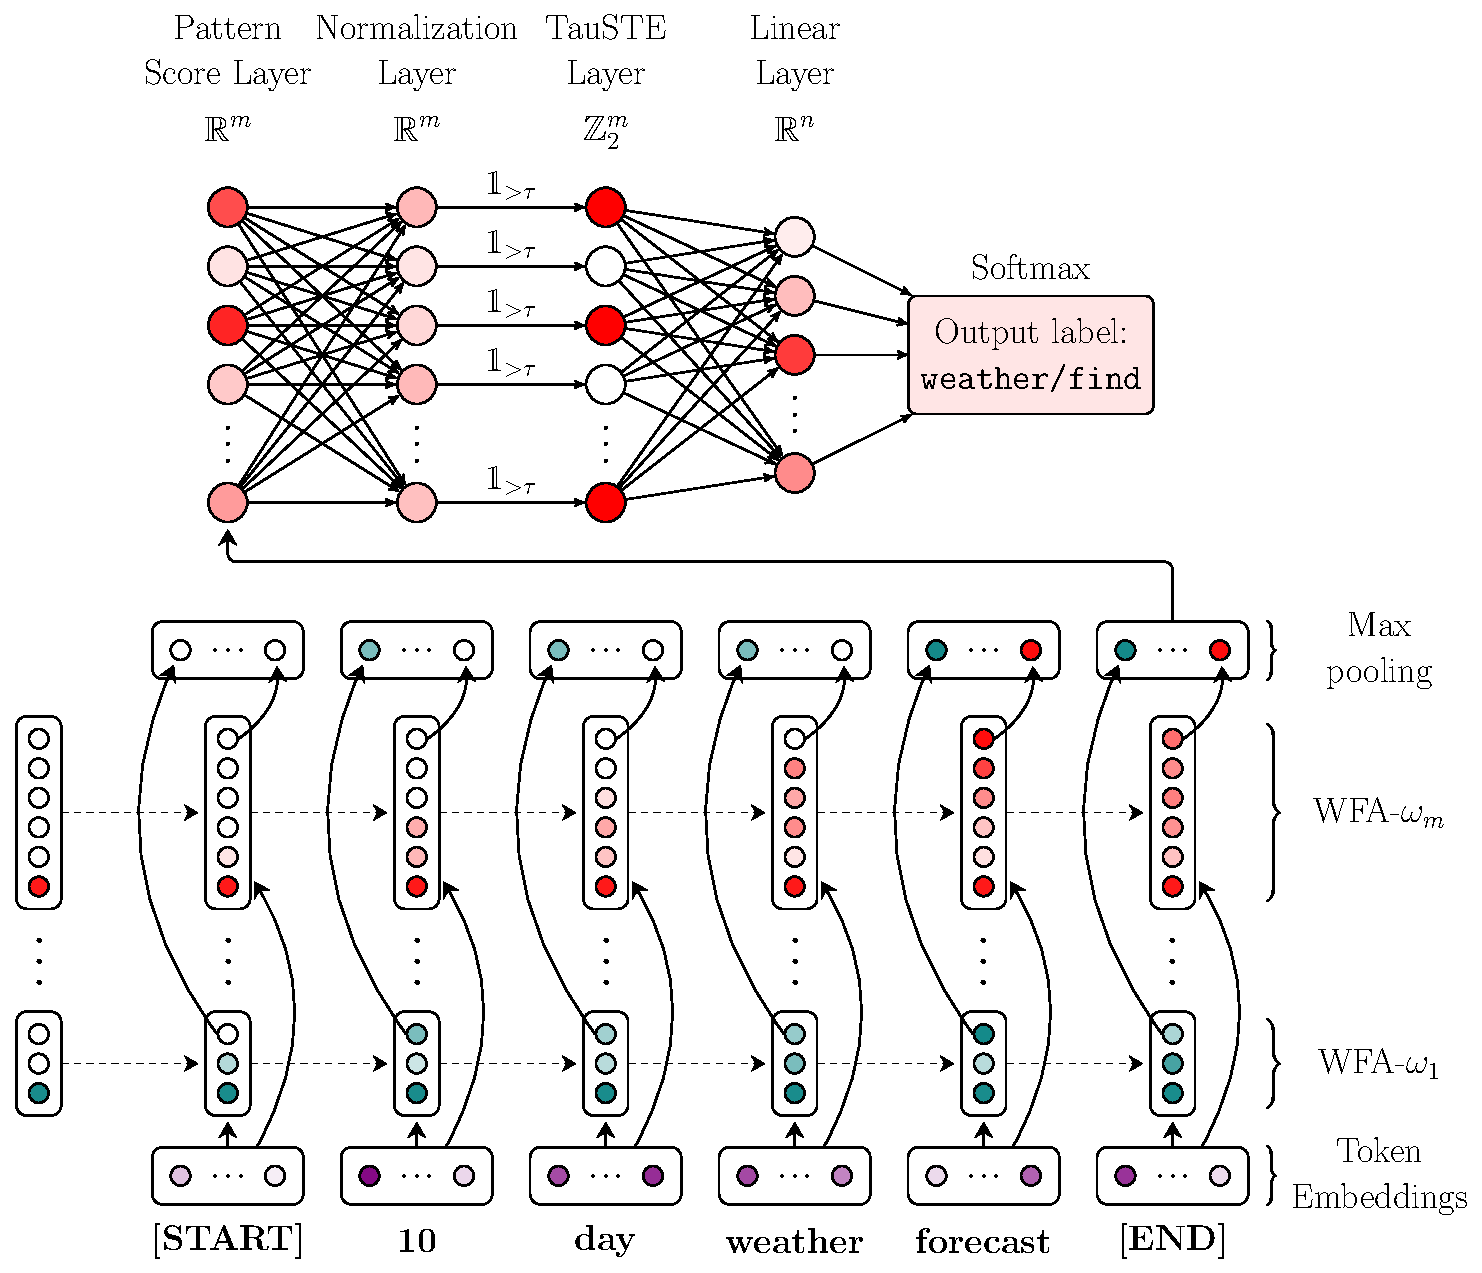
\includegraphics[width=8.5cm]{pdfs/generated/spp_computational_graph/main.pdf}};
      \path<1>[fill=white, fill opacity=0.7] (0,3.75) rectangle (7,7.3);
      \path<2>[fill=white, fill opacity=0.7] (3.125,4.1) rectangle (7,7.3);
      \path<3>[fill=white, fill opacity=0.7] (4,4.1) rectangle (7,7.3);
      \path<4>[fill=white, fill opacity=0.7] (0.1,0.1) rectangle (0.1,0.1);
      \path<5>[fill=white, fill opacity=0.7] (0,4.3) rectangle (3.125,7.3);
      \path<5>[fill=white, fill opacity=0.7] (3.85,4.3) rectangle (7,7.3);
    \end{tikzpicture}
    \caption{SoPa++ computational graph; flow of graph is
      from bottom to top and left to right}
    \label{fig:spp_computational_graph}
  \end{figure}
\end{frame}

\begin{frame}
  \frametitle{SoPa++: Regular Expression (RE) proxy}
  \begin{figure}
    \centering
    \begin{tikzpicture}
      \node[anchor=south west,inner sep=0] at (0,0) {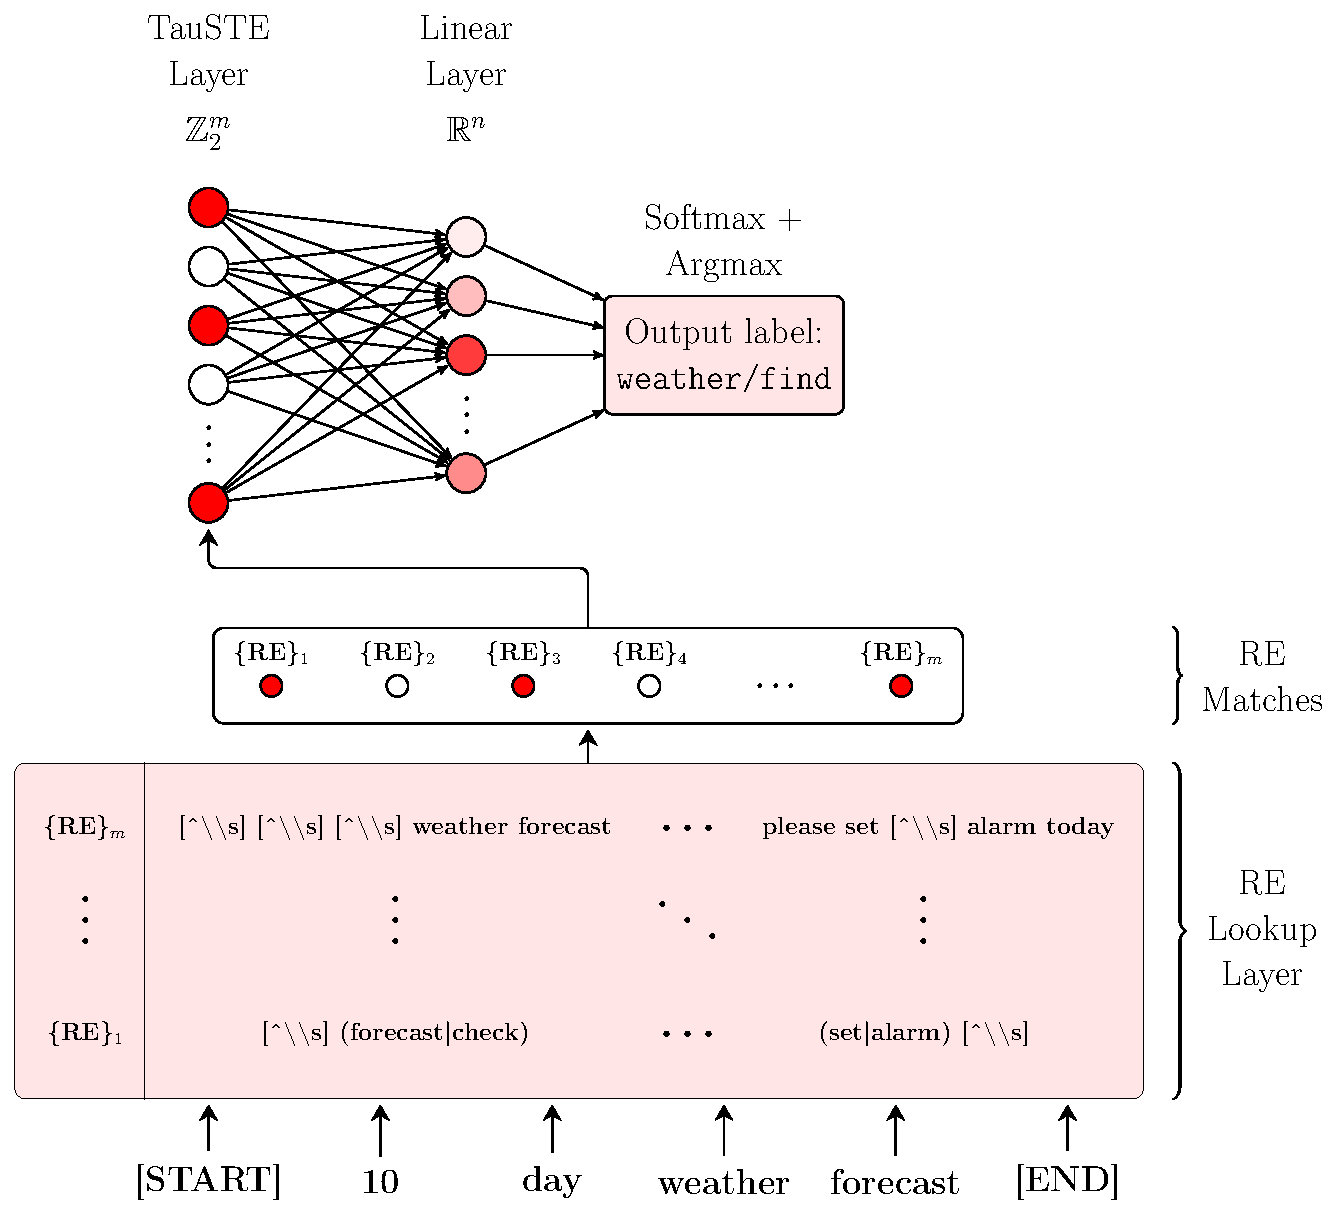
\includegraphics[width=8cm]{pdfs/generated/regex_computational_graph/main.pdf}};
      \path<1>[fill=white, fill opacity=0.7] (0,2.7) rectangle (8,7.2);
      \path<2>[fill=white, fill opacity=0.7] (0,3.525) rectangle (8,7.2);
      \path<3>[fill=white, fill opacity=0.7] (2,4.3) rectangle (8,7.2);
      \path<4>[fill=white, fill opacity=0.7] (0.1,0.1) rectangle (0.1,0.1);
    \end{tikzpicture}
    \caption{RE proxy computational graph; flow of graph is
      from bottom to top and left to right}
    \label{fig:regex_computational_graph}
  \end{figure}
\end{frame}

\begin{frame}
  \frametitle{SoPa vs. SoPa++}
  \begin{table}[t!]
    \centering \def\arraystretch{1.5}
    \begin{tabular}{L{0.275\linewidth} L{0.3\linewidth} L{0.3\linewidth}}
      \toprule
      Characteristic & SoPa & SoPa++ \\
      \midrule
      Text casing & True-cased & Lower-cased \\ 
      Token embeddings & GloVe 840B 300-dimensions & GloVe 6B 300-dimensions \\
      \uncover<2->{\textbf{WFAs} & Linear-chain WFA's with $\epsilon$, self-loop and main-path transitions & Strict linear-chain WFA-$\omega$'s with $\omega$ and main-path transitions} \\
      \uncover<3->{\textbf{Hidden layers} & Multi-layer perceptron after max-pooling & Layer normalization, TauSTE and linear transformation after max-pooling} \\
      \uncover<4> {\textbf{Post-hoc explainability technique(s)} & Local explanations, feature relevance & Explanations by simplification} \\
      \bottomrule
    \end{tabular}
    \caption{Summarized differences for SoPa vs. SoPa++}
    \label{tab:sopa_spp_comparison}
  \end{table}
\end{frame}

\begin{frame}
  \frametitle{Research Question 1: Competitive performance}
  \uncover<2>{\begin{table}[t!]
      \centering
      \begin{tabular}{lll}
        \toprule
        Model size & Patterns hyperparameter $P$ & Parameter count \\
        \midrule
        Small & \texttt{6-10\_5-10\_4-10\_3-10} & 1,260,292 \\
        Medium & \texttt{6-25\_5-25\_4-25\_3-25} & 1,351,612  \\
        Large & \texttt{6-50\_5-50\_4-50\_3-50} & 1,503,812 \\
        \bottomrule
      \end{tabular}
      \caption{Three different SoPa++ model sizes used during training}
      \label{tab:model_types}
    \end{table}}
  \begin{itemize}
    \setlength\itemsep{1em}
    \uncover<1>{\item RQ 1: Does SoPa++ provide \textbf{competitive} performance?
      \item Competitive accuracy range: \bm{$96.6-99.5\%$}
      \citep{schuster-etal-2019-cross-lingual,zhang2019joint,zhang-etal-2020-intent}}
    \uncover<2>{\item Upsampling minority classes to mitigate data imbalance
      \item Grid-search with three model sizes, varying $\tau$-thresholds: $\{0.00, 0.25, 0.50,
      0.75, 1.00\}$ and 10 random seed iterations
      \item $3 \times 5 \times 10 = 150$ model runs
      \item Evaluation and comparison on the test set}
  \end{itemize}
\end{frame}

\begin{frame}
  \frametitle{Research Question 2: Effective explanations by simplification}
  \begin{itemize}  
    \setlength\itemsep{1em}
    \uncover<1>{\item RQ 2: To what extent does SoPa++ contribute to \textbf{effective}
      explanations by simplification?
      \item Effective explanations by simplification require \textbf{simpler model},
      \textbf{similar performance} and \textbf{maximizing resemblance} to
      antecedent
      \item Similar performance $\Rightarrow$ compare test set evaluations
      \item Maximum resemblance $\Rightarrow$ minimum distances over test set}
    \uncover<2>{\item Softmax distance norm:
      \begin{equation*}
        \delta_{\sigma}(\bm{y}) = \left\Vert \bm{\sigma_{\mathcal{S}}} - \bm{\sigma_{\mathcal{R}}} \right\Vert_{2} = \sqrt{\sum^n_{i=1} (\sigma_{\mathcal{S}_i} - \sigma_{\mathcal{R}_i})^2} 
      \end{equation*}
      \item Binary-misalignment rate:
      \begin{equation*}
        \delta_b(\bm{y}) = \dfrac{\left\Vert \bm{b_{\mathcal{S}}} - \bm{b_{\mathcal{R}}} \right\Vert_{1}}{dim(\bm{b_{\mathcal{S}}} - \bm{b_{\mathcal{R}}})} = \dfrac{\sum^n_{i=1} |b_{\mathcal{S}_i} - b_{\mathcal{R}_i}|}{{dim(\bm{b_{\mathcal{S}}} - \bm{b_{\mathcal{R}}})}}
      \end{equation*}}
  \end{itemize}
\end{frame}

\begin{frame}
  \frametitle{Research Question 3: Interesting and relevant explanations}
  \begin{itemize}
    \setlength\itemsep{2em}
    \uncover<1>{\item RQ 3: What \textbf{interesting and relevant} explanations can SoPa++
      provide?
      \item Open-ended question, can answer in different ways}
    \uncover<2>{\item Capitalize on the new linear layer $\Rightarrow$ allows for direct
      analysis of relative linear weights
      \item Sample REs from RE lookup layer corresponding to salient TauSTE
      neurons
      \item Analyze REs for interesting linguistic features and inductive biases}
  \end{itemize}
\end{frame}

\section{Results}

\begin{frame}
  \frametitle{Research Question 1: Competitive performance}
  \centering
  \uncovergraphics<1->[width=9cm,valign=t]{pdfs/generated/train_spp_grid_1624885671.pdf}
  \captionof{figure}{Validation accuracies of SoPa++ models against training updates}
  \label{fig:results_training}

  \uncover<2>{\begin{table}
      \centering \def\arraystretch{1.3}
      \tiny
      \begin{tabular}{lllllll}
        \toprule
        && \multicolumn{5}{c}{Accuracy in $\%$ with mean $\pm$ standard-deviation} \\[2pt]
        \cline{3-7} \\[-7pt]
        Size & Parameters & $\tau$=0.00 & $\tau$=0.25 & $\tau$=0.50 & $\tau$=0.75 & $\tau$=1.00 \\
        \midrule
        Small & 1,260,292 & \bm{$97.6 \pm 0.2$} & 97.6 $\pm$ 0.2 & 97.3 $\pm$ 0.2 & 97.0 $\pm$ 0.3 & 96.9 $\pm$ 0.3 \\
        Medium & 1,351,612 & \bm{$98.3 \pm 0.2$} & 98.1 $\pm$ 0.1 & 98.0 $\pm$ 0.2 & 97.9 $\pm$ 0.1 & 97.7 $\pm$ 0.1  \\
        Large & 1,503,812 & \bm{$98.3 \pm 0.2$} & 98.3 $\pm$ 0.2 & 98.2 $\pm$ 0.2 & 98.1 $\pm$ 0.2 & 98.0 $\pm$ 0.2 \\
        \bottomrule
      \end{tabular}
      \caption{Test accuracies of SoPa++ models}
      \label{tab:results_evaluation}
    \end{table}}
\end{frame}

\begin{frame}
  \frametitle{Research Question 2: Effective explanations by simplification}
  \begin{figure}
    \centering
    \begin{tikzpicture}
      \node[anchor=south west,inner sep=0] at (0,0)
      {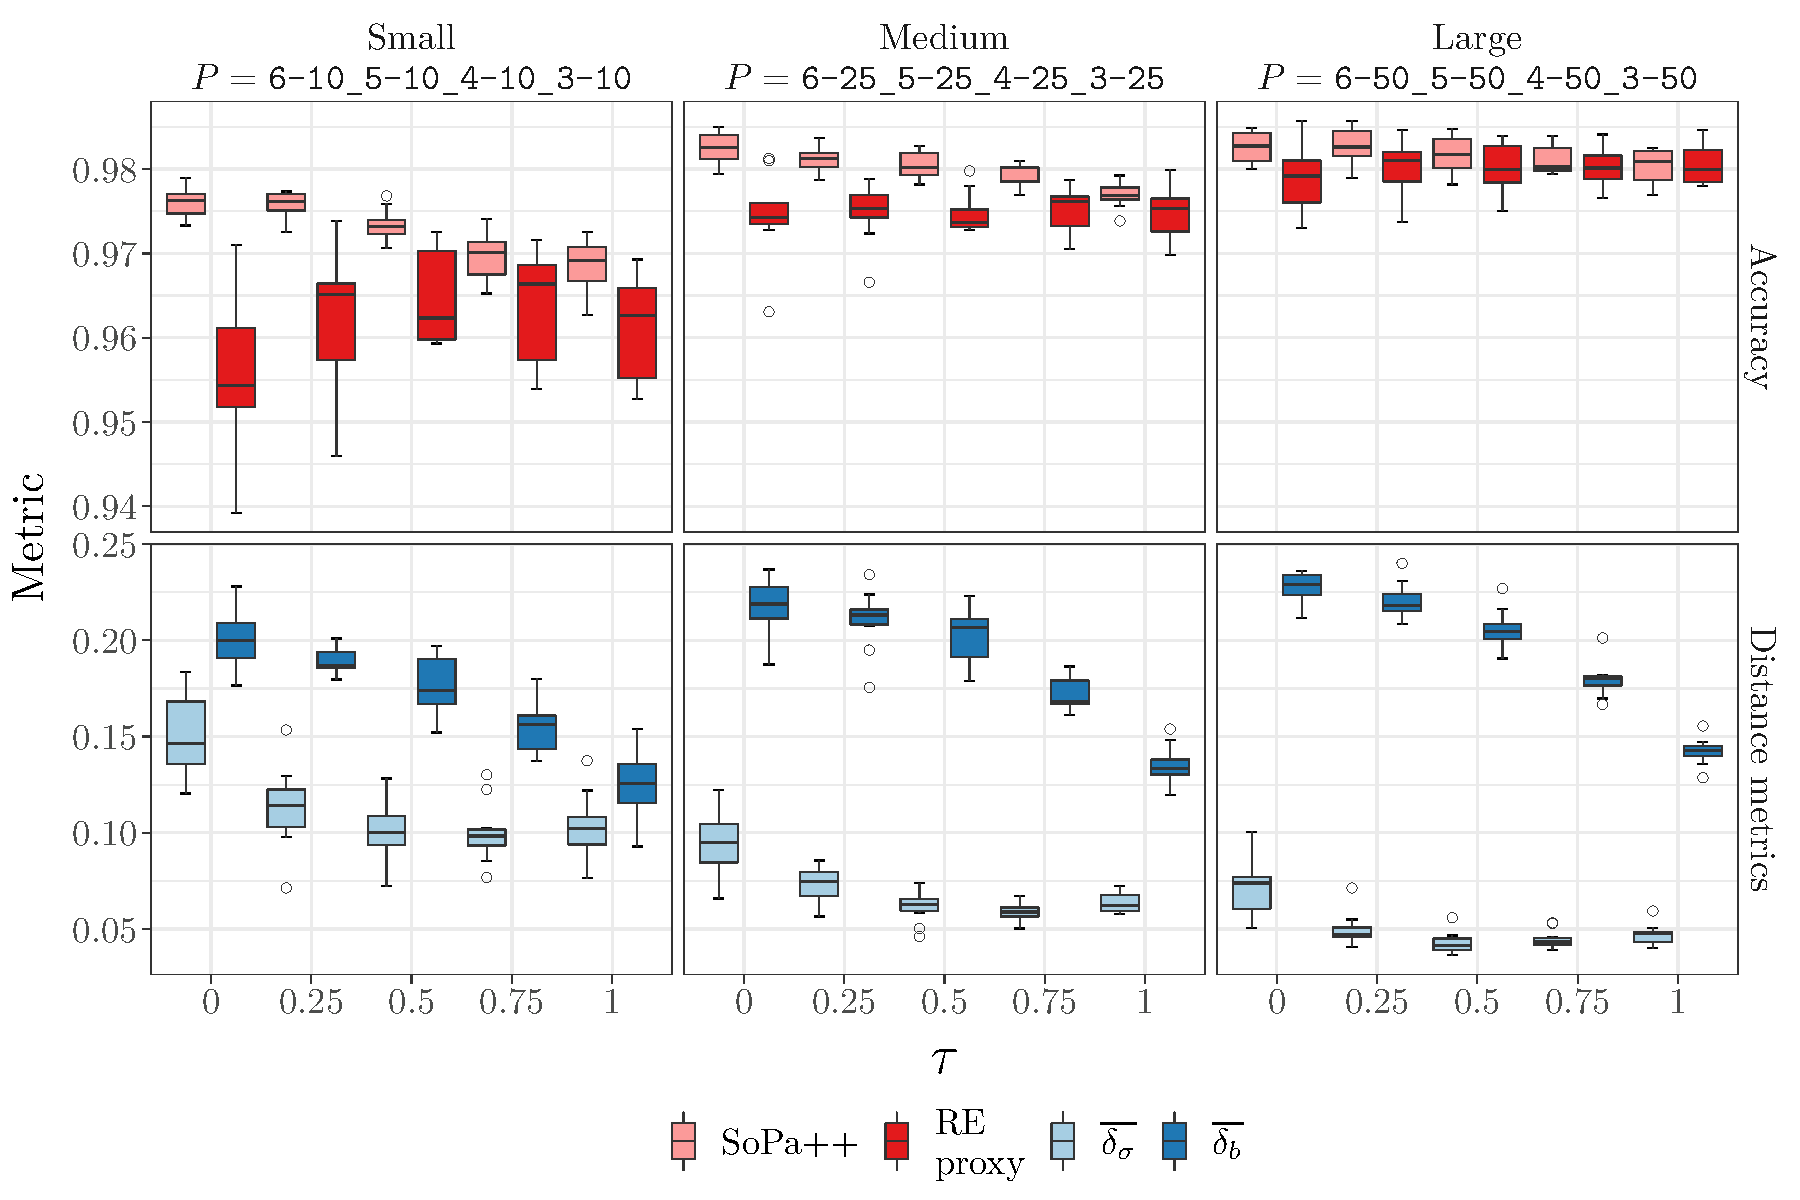
\includegraphics[width=10.5cm]{pdfs/generated/evaluate_spp_grid_1618059389.pdf}
      };
      \path<1>[fill=white, fill opacity=0.7] (0.4,1) rectangle (10.5,3.9);
      \path<2>[fill=white, fill opacity=0.7] (0.4,3.9) rectangle (10.5,7);
    \end{tikzpicture}
    \caption{Visualization of model-pair accuracies and distance metrics}
    \label{fig:explain_evaluate}
  \end{figure}
\end{frame}

\begin{frame}
  \frametitle{Research Question 3: Interesting and relevant explanations}
  \begin{figure}
    \centering
    \begin{tikzpicture}
      \node[anchor=south west,inner sep=0] at (0,0) {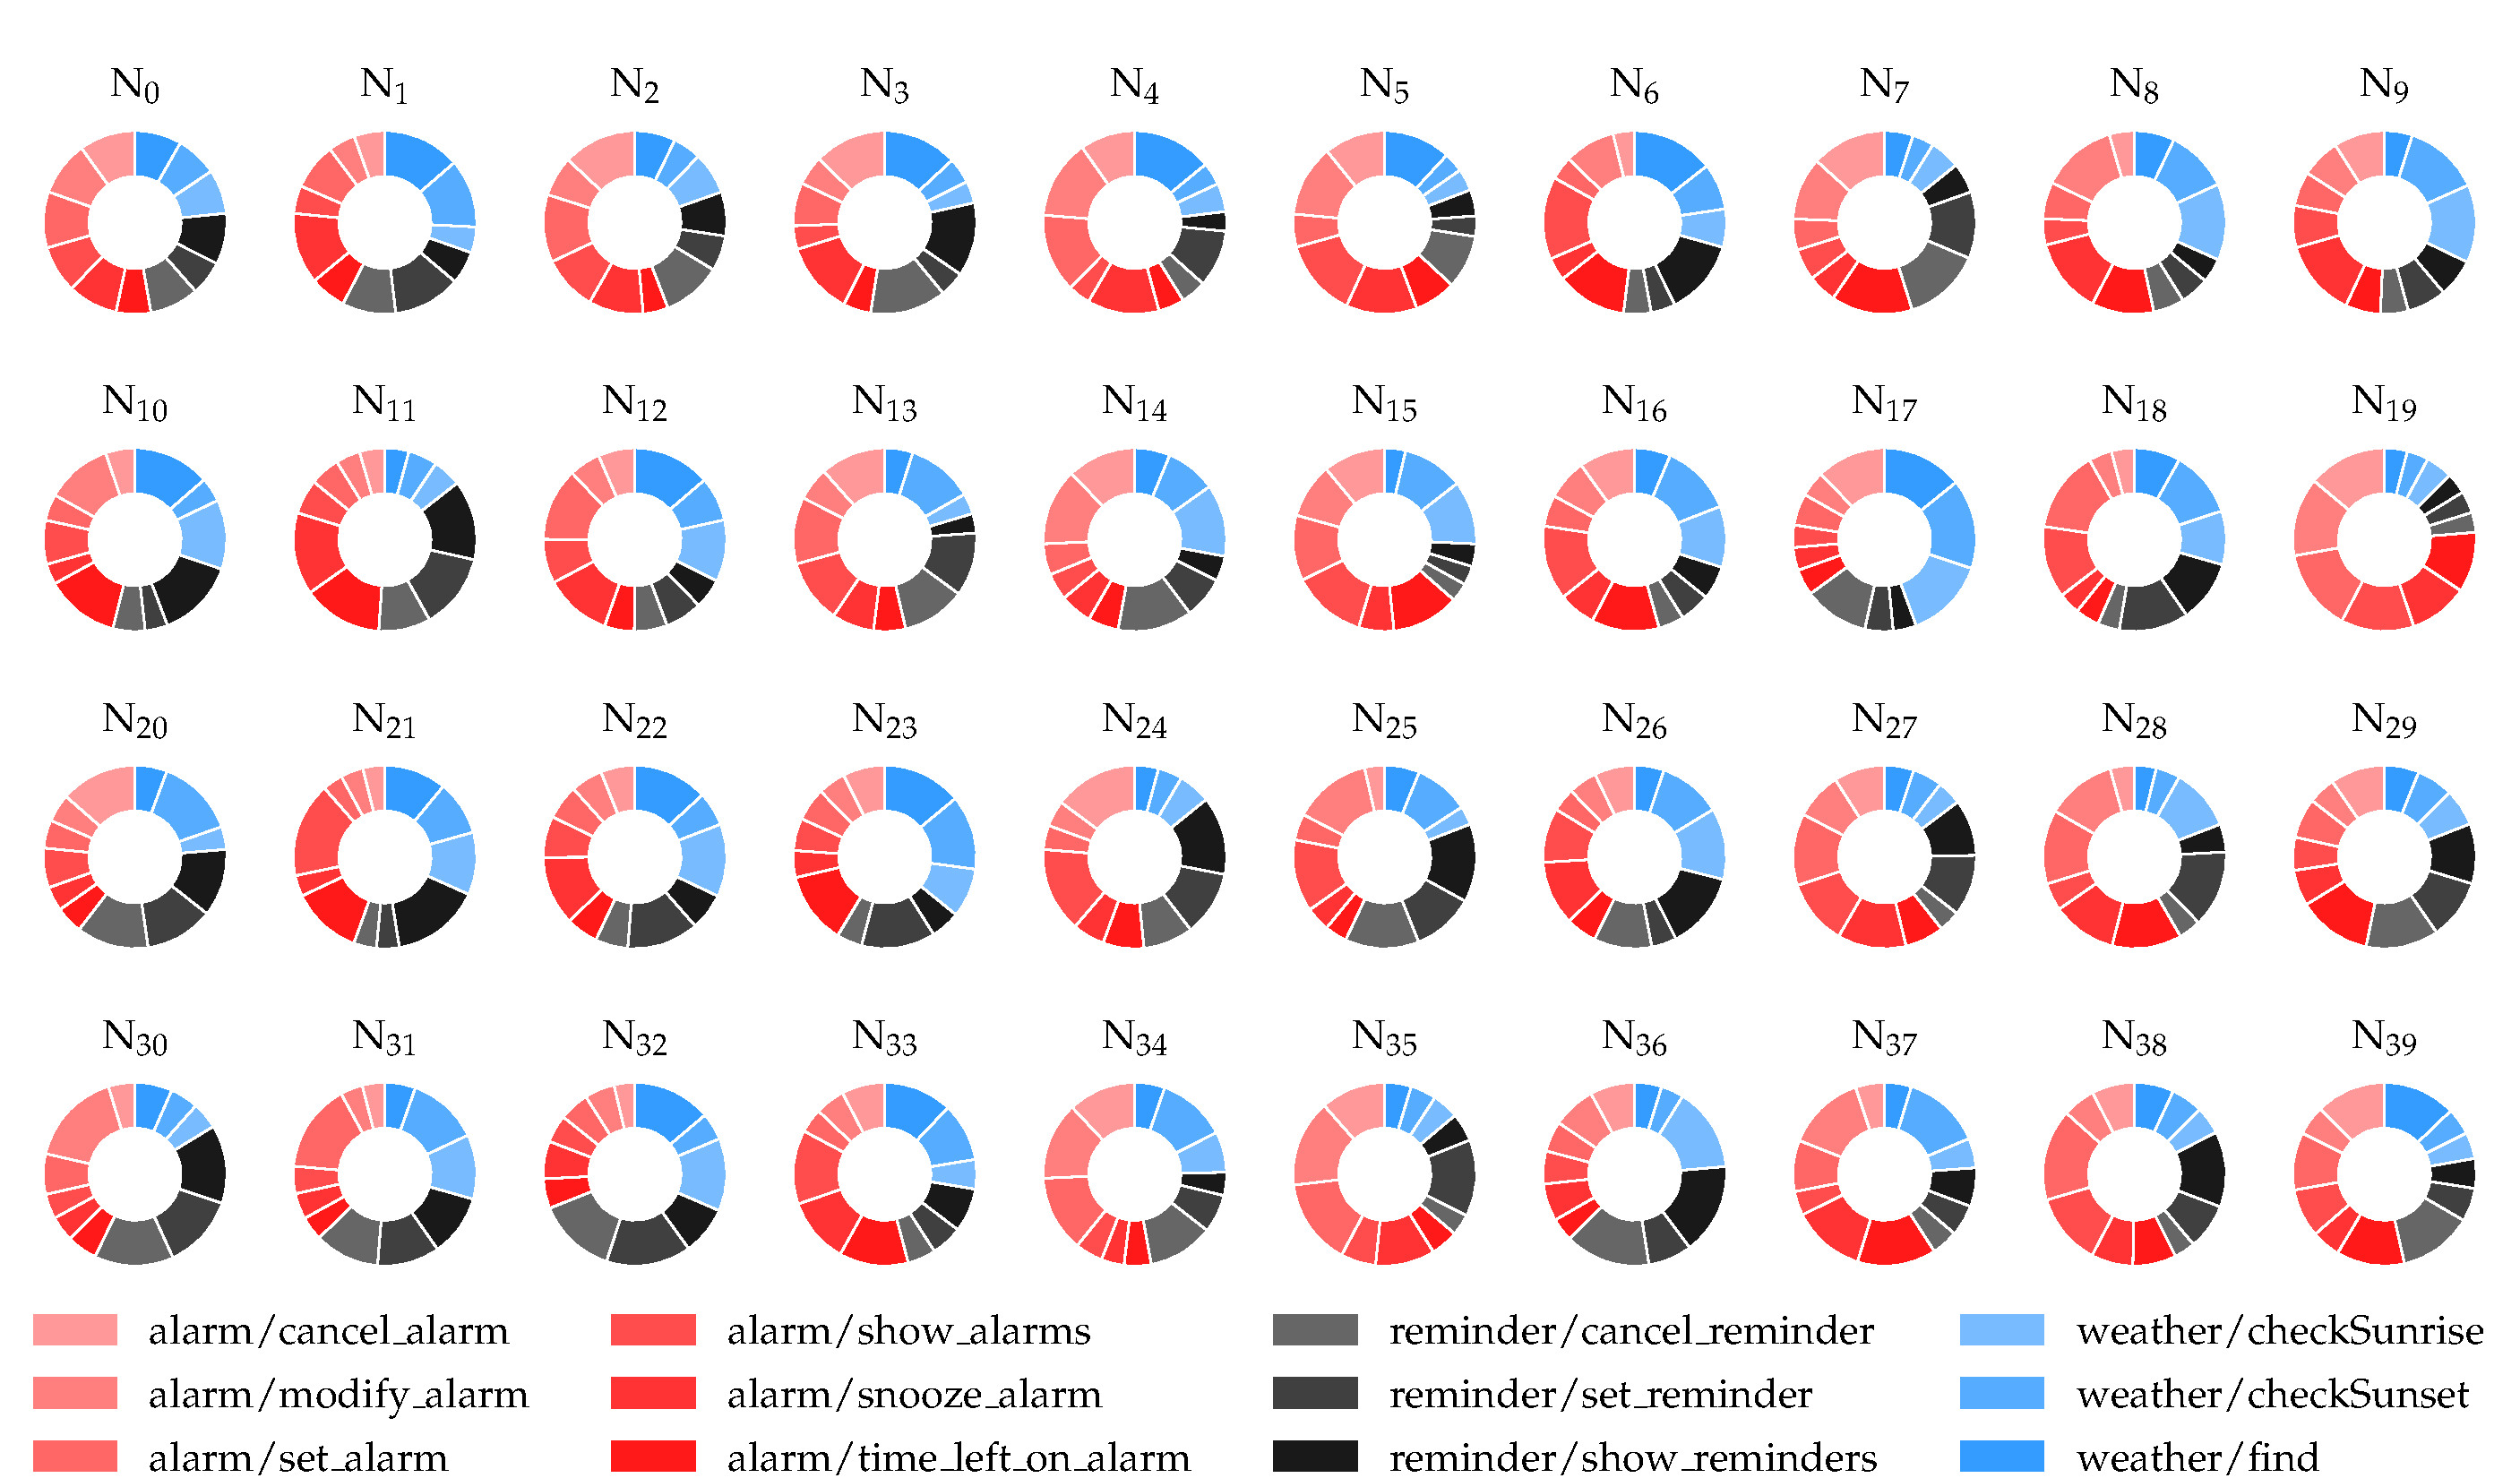
\includegraphics[width=10cm]{pdfs/generated/neurons_1618067685.pdf}};
      \path<1>[fill=white, fill opacity=0.7] (0,0.7) rectangle (10,5.65);
      \draw<3>[red] (7,3.2) rectangle (8,4.45);
    \end{tikzpicture}
    \vspace{5pt}
    \caption{Relative linear layer weights applied to TauSTE neurons for the best
      performing small RE proxy model with a test accuracy of 97.4$\%$}
    \label{fig:neuron_weights}
  \end{figure}
\end{frame}

\begin{frame}
  \frametitle{Research Question 3: Interesting and relevant explanations}
  \begin{figure}
    \centering 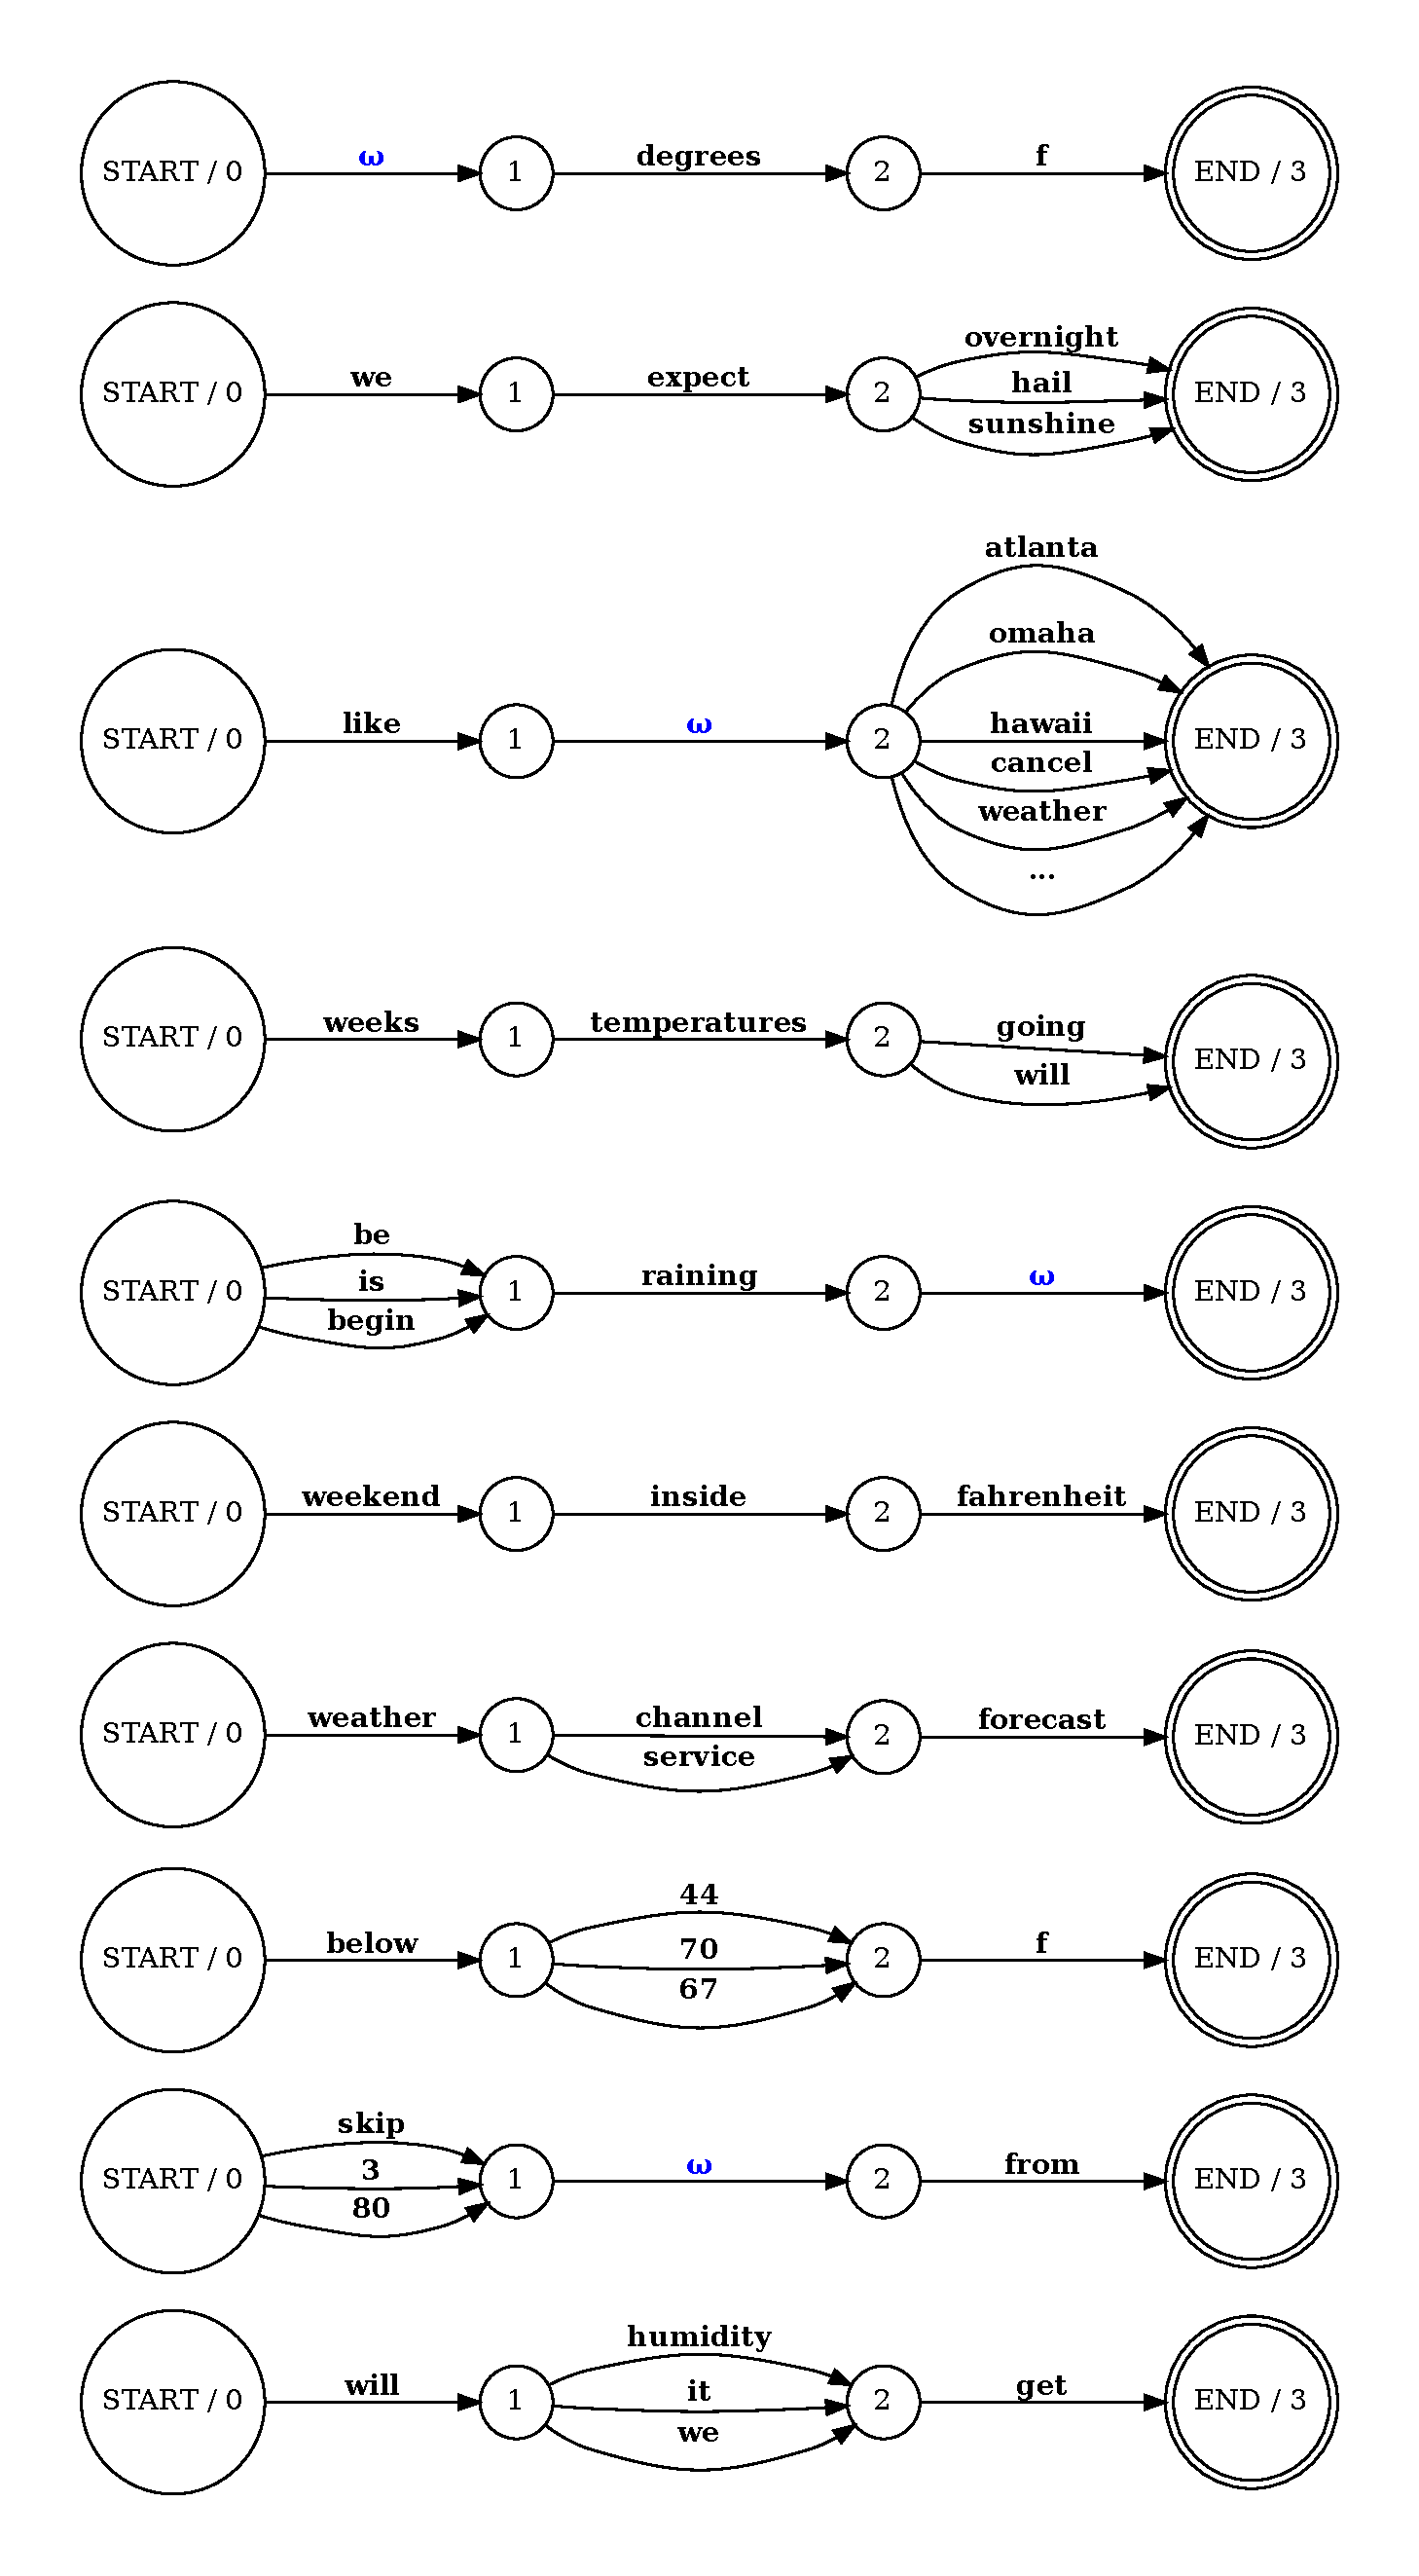
\includegraphics[trim={1.1cm 20.5cm 1.1cm
      1.1cm},clip,height=4.9cm,valign=t]{pdfs/generated/neurons_regex_1618067722/activating_regex_sample_17.pdf}
    \hfill 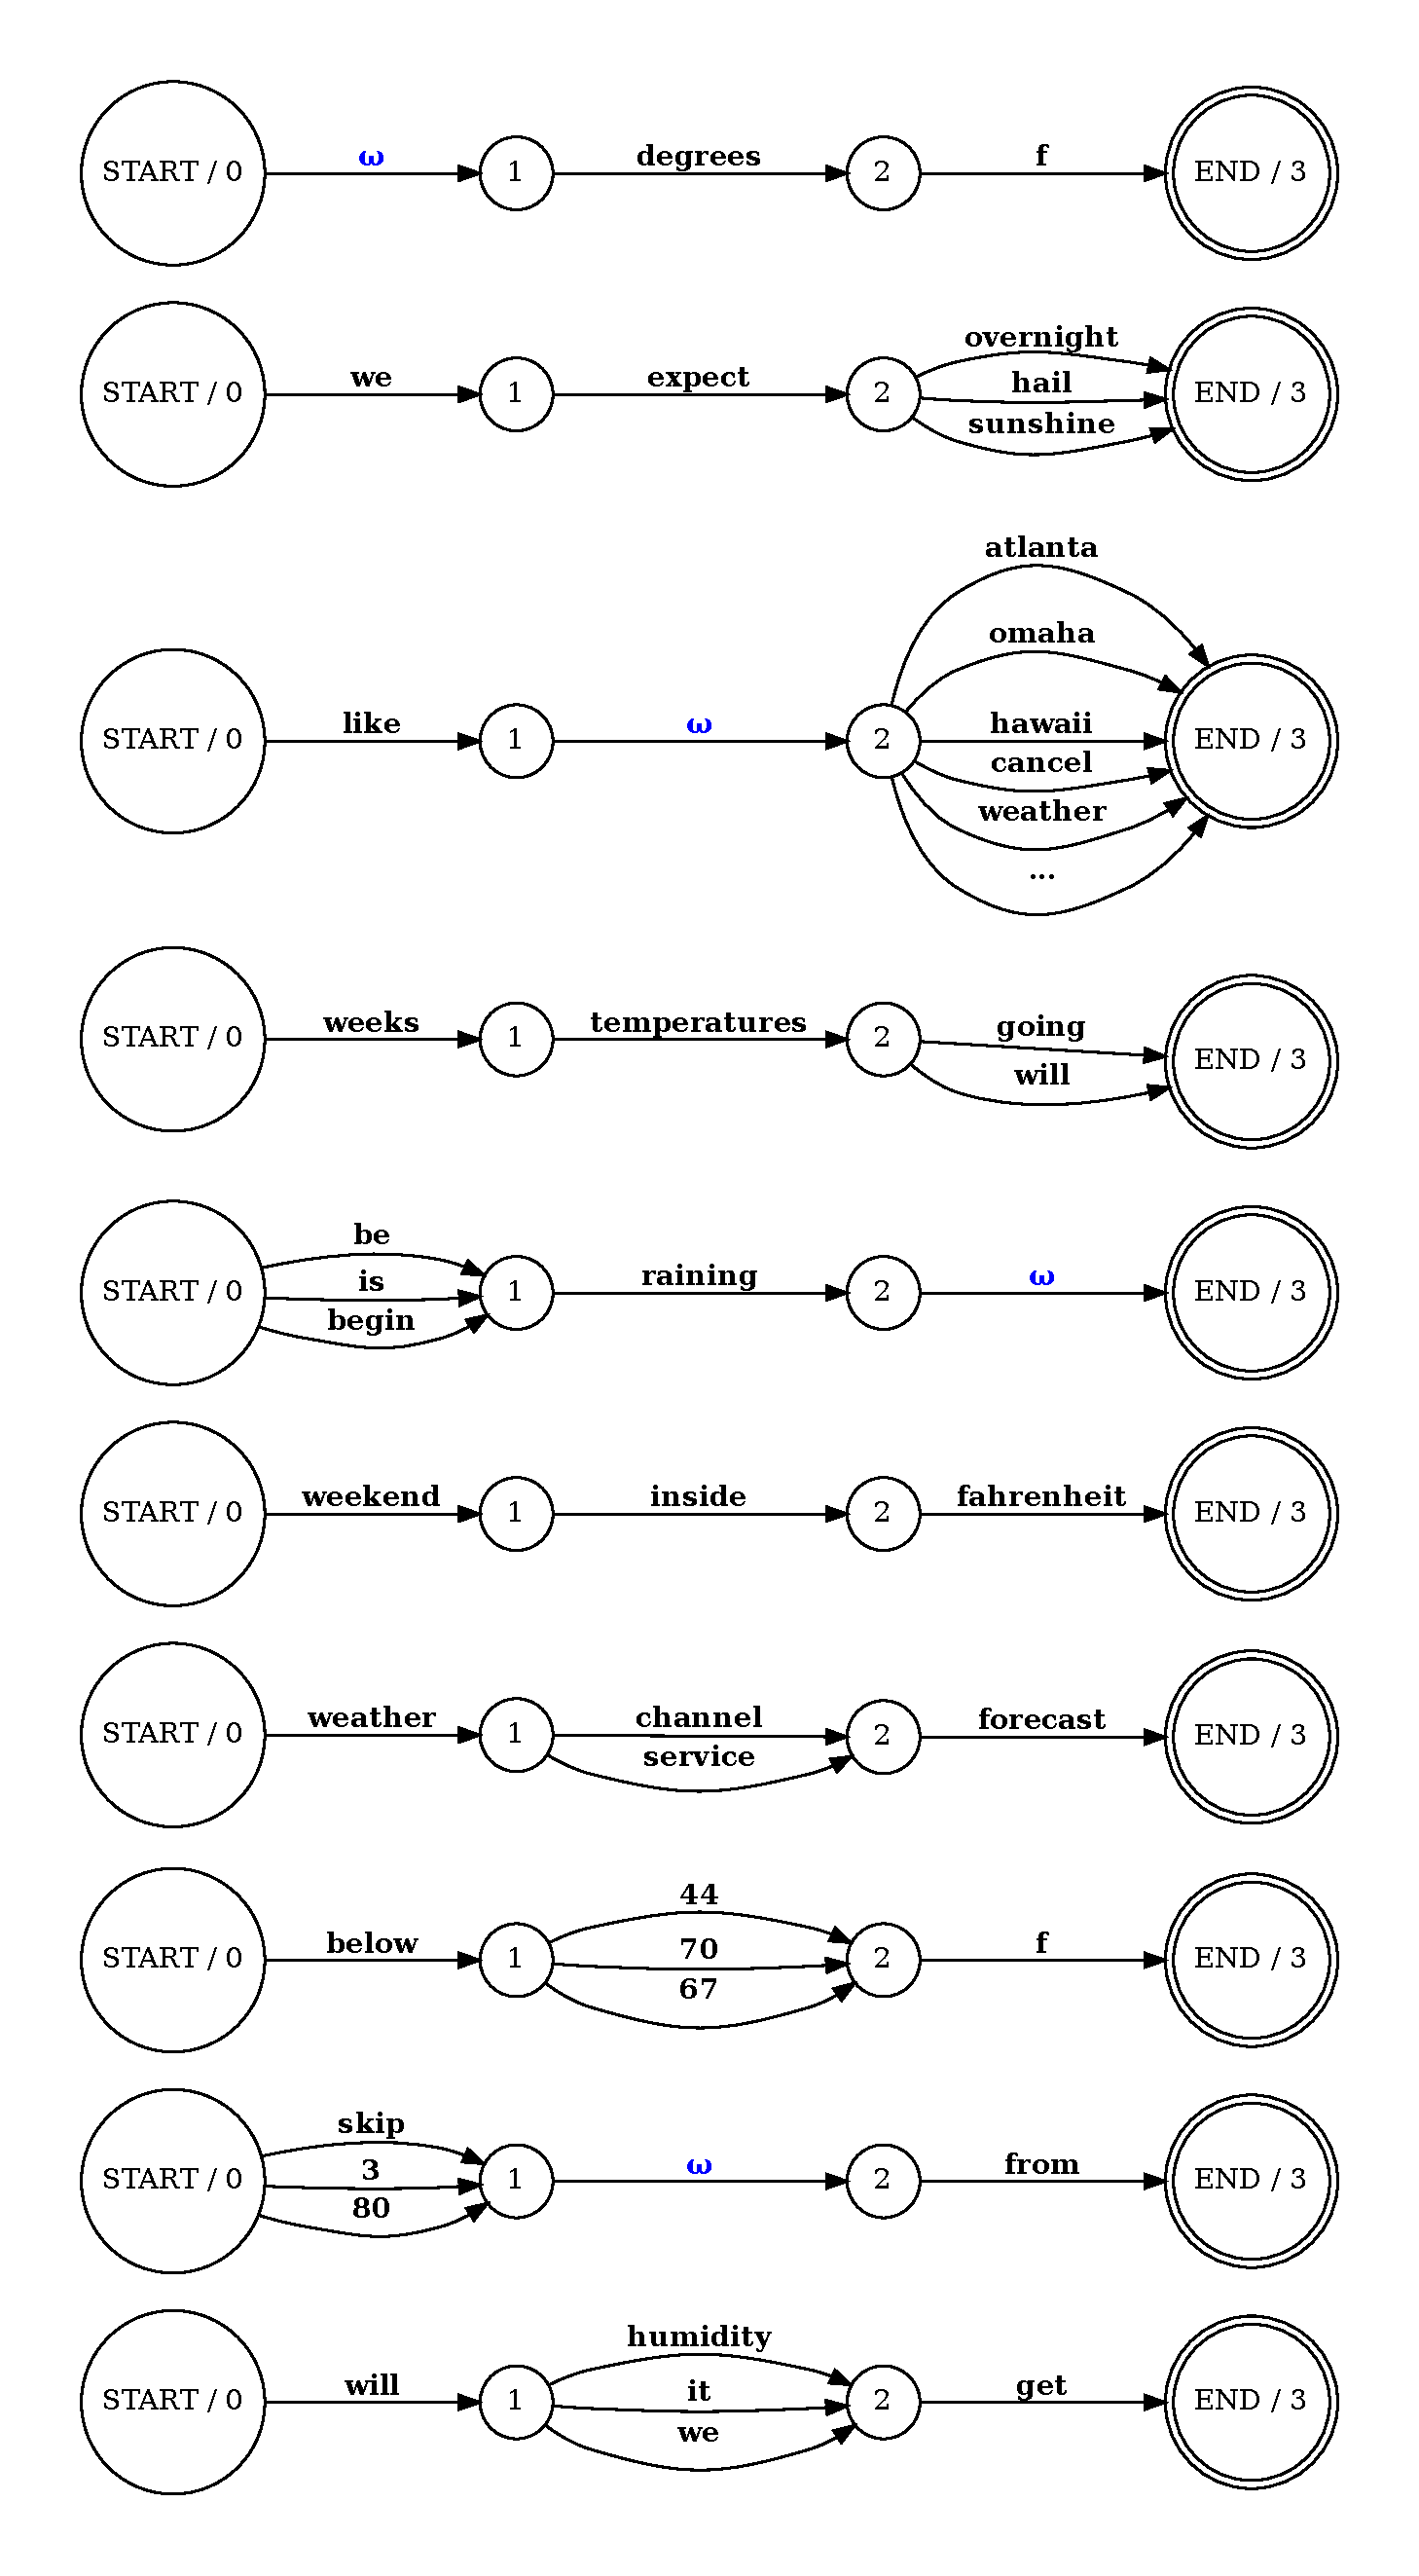
\includegraphics[trim={1.1cm 1.1cm 1.1cm
      24.5cm},clip,height=4.9cm,valign=t]{pdfs/generated/neurons_regex_1618067722/activating_regex_sample_17.pdf}
    \vspace{5pt}
    \caption{Ten sampled regular expressions from the RE lookup layer
      corresponding to TauSTE neuron 17 for the best performing small RE proxy
      model}
    \label{fig:regex_example_neuron_weather}
  \end{figure}
\end{frame}

\section{Discussion}

\begin{frame}
  \frametitle{Research Question 1: Competitive performance}
  \uncover<1->{Overview: \setlength{\leftmargini}{0.5cm}
    \begin{itemize}
      \setlength\itemsep{1em}
      \item RQ 1: Does SoPa++ provide \textbf{competitive} performance?
      \item Competitive accuracy range: $96.6-99.5\%$
      \citep{schuster-etal-2019-cross-lingual,zhang2019joint,zhang-etal-2020-intent} 
      \item Observed best accuracy range for $\tau=0.00$: \bm{$97.6-98.3\%$}
      \item SoPa++ offers \textbf{competitive} performance on FMTOD's English language
      intent detection task
    \end{itemize}}

  \vspace{15pt}
  
  \uncover<2>{Discussion: \setlength{\leftmargini}{0.5cm}
    \begin{itemize}
      \setlength\itemsep{1em}
      \item Other studies worked with true-cased text 
      \item Observed performance is in the middle of competitive range
      \item Worth noting the sizes of competitive BERT-derived models with
      external data
    \end{itemize}}
\end{frame}

\begin{frame}
  \frametitle{Research Question 2: Effective explanations by simplification}
  \uncover<1->{Overview: \setlength{\leftmargini}{0.5cm}
    \begin{itemize}
      \setlength\itemsep{1em}
      \item RQ 2: To what extent does SoPa++ contribute to \textbf{effective}
      explanations by simplification?
      \item Effective explanations by simplification require simpler model,
      similar performance and maximizing resemblance to antecedent
      \item \textbf{Effective} to the extent of: lowest accuracy differences ranging
      from \bm{$0.1-0.7\%$} and softmax distance norms ranging from \bm{$4.3-10.0\%$}
      \item Most effective for medium-large sized models with $\tau \in [0.50, 1.00]$
    \end{itemize}}

  \vspace{15pt}
  
  \uncover<2>{Discussion: \setlength{\leftmargini}{0.5cm}
    \begin{itemize}
      \setlength\itemsep{1em}
      \item No benchmark for effective explanations by simplification
      \item RE proxy may not necessarily always be transparent given size of RE
      lookup layer
      \item Target audience was omitted in this analysis
    \end{itemize}}
\end{frame}

\begin{frame}
  \frametitle{Research Question 3: Interesting and relevant explanations}
  \uncover<1->{Overview: \setlength{\leftmargini}{0.5cm}
    \begin{itemize}
      \setlength\itemsep{1em}
      \item RQ 3: What \textbf{interesting and relevant} explanations can SoPa++
      provide?
      \item Similar lexical properties in branches
      \item USA-centric inductive biases
      \item Pronoun-level inductive biases
    \end{itemize}}

  \vspace{10pt}
  
  \uncover<2->{Discussion:}
  \begin{figure}
    \centering 
    \uncovergraphics<2>[trim={1.1cm 28.5cm 1.1cm
      9cm},clip,width=5cm]{pdfs/generated/neurons_regex_1618067722/activating_regex_sample_17.pdf}
    \raisebox{0.37cm}{\uncovergraphics<3>[trim={1.1cm 9cm 1.1cm
        32cm},clip,width=5cm]{pdfs/generated/neurons_regex_1618067722/activating_regex_sample_17.pdf}}
    \vspace{5pt}
    \uncovergraphics<4>[trim={1.1cm 1.1cm 1.1cm
      40cm},clip,width=5cm]{pdfs/generated/neurons_regex_1618067722/activating_regex_sample_17.pdf} 
    \uncover<2->{\caption{Sampled regular expressions from the RE lookup layer
        corresponding to TauSTE neuron 17 for the best performing small RE proxy
        model}}
    \label{fig:regex_more_examples}
  \end{figure}
\end{frame}

\section{Conclusions}
\begin{frame}
  \frametitle{Conclusions}
  Objective: \setlength{\leftmargini}{0.5cm}
  \begin{itemize}
    \item Address limitations of SoPa by proposing \textbf{SoPa++}, which could
    allow for effective explanations by simplification
    \uncover<2->{\large\color{ForestGreen}\checkmark}
  \end{itemize}
  
  \vspace{15pt}

  Research questions:
  \begin{enumerate}
    \setlength\itemsep{1.5em}
    \item Does SoPa++ provide \textbf{competitive} performance? \uncover<3->{
      \begin{itemize}
        \item Best accuracy range: \bm{$97.6-98.3\%$}
        \large\color{ForestGreen}\checkmark
      \end{itemize}}
    \item To what extent does SoPa++ contribute to \textbf{effective}
    explanations by simplification?
    \begin{itemize}
      \setlength\itemsep{0.5em} \uncover<4->{
        \item Lowest accuracy differences ranging from \bm{$0.1-0.7\%$} and
        softmax distance norms ranging from \bm{$4.3-10.0\%$}
        {\large\color{ForestGreen}\checkmark}} \uncover<5->{
        \item Target audience analysis omitted {\large\color{orange}\ding{55}}}
    \end{itemize}
    \item What \textbf{interesting and relevant} explanations can SoPa++
    provide?
    \begin{itemize}
      \setlength\itemsep{0.5em} \uncover<6->{\item Regular expression samples
        from salient TauSTE neurons analyzed
        {\large\color{ForestGreen}\checkmark}
        \item Linguistic features and inductive biases
        {\large\color{ForestGreen}\checkmark}} \uncover<7->{\item Small sample
        size {\large\color{orange}\ding{55}}}
    \end{itemize}
  \end{enumerate}
\end{frame}

\section{Further work}

\begin{frame}
  \frametitle{Further work}
  \uncover<1>{ Explainability: \setlength{\leftmargini}{0.5cm}
    \begin{itemize}
      \setlength\itemsep{0.5em}
      \item Are SoPa++'s explanations \textbf{useful} for its target audience?
    \end{itemize}
  }

  \vspace{10pt}
  
  \uncover<2>{ Bias correction:
    \begin{itemize}
      \setlength\itemsep{0.5em}
      \item Manual bias corrections through large-scale analysis of RE lookup layer
      \item Mitigate \textbf{ethical} issues of using black-box models?
    \end{itemize}
  }
  
  \vspace{10pt}

  \uncover<3>{ Generalization:
    \begin{itemize}
      \setlength\itemsep{0.5em}
      \item Possible to generalize branches with broad categories like
      locations and numbers
      \item For example, replace digital tokens with
      \texttt{\textbackslash-?[\textbackslash d]+\textbackslash
        .?[\textbackslash d]*}
      \item \textbf{Robustness} on unseen data?
    \end{itemize}
  }

  \vspace{10pt}
  
  \uncover<4>{ Efficiency:
    \begin{itemize}
      \setlength\itemsep{0.5em}
      \item \textbf{Parallelize} RE lookup layer
      \item Utilize GPU-based regular expression matching algorithms
      \citep{wang2011gregex,zu2012gpu,yu2013gpu}
    \end{itemize}
  } 
\end{frame}

\begin{frame}{}
  \frametitle{\null}
  \centering
  \Huge
  \textit{Thank you for your time and attention} \ensuremath\heartsuit
\end{frame}

\begin{frame}[allowframebreaks]
  \frametitle{Bibliography} \printbibliography[title = {Bibliography}]
\end{frame}

\end{document}

% LocalWords:  explainability Atreya Shankar Sharid Loáiciga nd Müller SoSe NLP% LocalWords:  WFA
% LocalWords:  Semiring semiring Semirings SoPa's WFAs preprocessed TauSTE STEs
% LocalWords:  TauSTE's embeddings GloVe WFA's perceptron hyperparameter RQ REs
% LocalWords:  Upsampling Softmax accuracies FMTOD's softmax centric SOTA NLP
% LocalWords:  Parallelize XAI FMTOD TOC
